% !TEX root = main.tex

\chapter{$\SCCP$}
\label{chapter.sccp}      

La Programaci\'on Concurrente por Restricciones (del ingl\'es, \textit{Concurrent Constraint Programming}, abreviado \textbf{\CCP}) es un modelo computacional en el cual agentes (v.gr., procesos, usuarios) interact\'uan sobre un banco de informaci\'on compartido, el cual puede contener informaci\'on parcial. Este modelo hace uso de dos operaciones b\'asicas, la operaci\'on $\ask$ intenta inferir si es posible obtener informaci\'on de los procesos, mientras que la operaci\'on $\tell$ agrega informaci\'on parcial al banco de los procesos. La notaci\'on cl\'asica de las operaciones \textit{read} and \textit{write} es reemplazada en este modelo por la notaci\'on $\ask$ and $\tell$. 

Las caracter\'isticas de \textbf{\CCP} lo identifican como un formalismo declarativo que permite la implementaci\'on de diferentes sistemas reactivos. En esta \'area \textbf{\CCP} se ha extendido para modelar diferentes tipos de concurrencia y abordar problemas que surgen en la modelaci\'on de sistemas reactivos. Dichas extensiones incluyen no-determinismo~\cite{Nielsen:2002:TCC:643009.643014}, movilidad y comportamiento sincronizado. La extensi\'on mas reciente agrega modalidades epist\'emicas y espaciales que permiten modelar comportamiento distribuido, que no era posible modelar con las extensiones anteriormente mencionadas.

Este cap\'itulo presenta algunas definiciones particulares requeridas para posteriormente definir las extensiones del modelo \textbf{\CCP}. Para m\'as informaci\'on se refiere el lector a~\cite{knight:hal-00761116}. La Secci\'on~\ref{srs.sccp} presenta el Sistema de Restricciones Simples. Las secciones~\ref{ser.sccp} y~\ref{sepr.sccp} presentan el sistema espacial y epist\'emico de restricciones, respectivamente, y sus propiedades. La secci\'on~\ref{ecp.sccp} presentan $\SCCP$ y \ECCP, dos variaciones del modelo \CCP. Finalmente, la Secci\'on~\ref{soe.sccp} presenta la sem\'antica operacional estructurada para espacios y conocimiento en procesos.

% Secci\'on: Sistema de restricciones simple
\section{Sistema de restricciones simple}
\label{srs.sccp}

El modelo \textbf{\CCP} es param\'etrico en un sistema de restricciones (del ingl\'es, \textit{Constraint System}, abreviado \textit{CS}). Esto significa que los par\'ametros del modelo de procesos son restricciones en alg\'un lenguaje de primer orden. El \textit{CS} es la estructura que especifica las interdependencias de la informaci\'on usada en el banco compartido por medio de f\'ormulas. 

De acuerdo con~\cite{DEBOER199537} las restricciones del sistema se pueden ver como un ret\'iculo algebraico completo. Este ret\'iculo es provisto de un orden parcial $\sqsubseteq$. Los detalles de un \textit{CS} se introducen en la Definici\'on~\ref{def:CS}.

\begin{definition}\label{def:CS}
Un \textit{sistema de restricciones} es un ret\'iculo algebraico completo \[C = (Con, Con_0, \sqsubseteq, \sqcup, \textit{true}, \textit{false})\] donde $Con$ es el conjunto de restricciones, $Con_0$ es el conjunto de elementos compactos de $Con$ y est\'a ordenado con respecto a $\sqsubseteq$, $\sqcup$ es la operaci\'on del l\'imite inferior definido en subconjuntos, y $true$ y $false$ son los elementos m\'inimo y m\'aximo de $Con$, respectivamente. 
\end{definition}

% Secci\'on: Sistema espacial de restricciones 
\section{Sistema espacial de restricciones}
\label{ser.sccp}

Para \textbf{$\SCCP$} es necesario definir un sistema espacial de restricciones, los cuales corresponden a una extensi\'on de \CS. El objetivo de $\SCCP$ es modelar un sistema distribuido de m\'ultiples agentes en el que cada agente tiene su propio espacio de computaci\'on. Esto se obtiene agregando la noci\'on de espacio para un agente, denotado por una funci\'on $\sfunc{c}_i$, que significa que una restricci\'on $c$ esta contenida en el espacio del agente $i$. La definici\'on de un \textit{sistema espacial de restricciones de $n$ agentes} se presenta en la Definici\'on~\ref{def:SCS}.

\theoremstyle{definition}
\begin{definition}\label{def:SCS}
Un \textit{sistema espacial de restricciones de $n$ agentes} (del ingl\'es, \textit{Spatial Constraint System}, abreviado $n$-SCS) es un sistema de restricciones \textbf{C} provisto con $n$ funciones ($\sfunc{\cdot}_1, \mathellipsis,\sfunc{\cdot}_n$) sobre el conjunto de restricciones \textit{Con}.  Cada funci\'on $\sfunc{\cdot}_i: Con \rightarrow Con$ debe satisfacer las siguientes propiedades: 
\begin{enumerate} 
	\item [\it{S.1}] \ $\sfunc{true}_i=true$
	\item [\it{S.2}] \ $\sfunc{c\sqcup d}_i=\sfunc{c}_i \sqcup \sfunc{d}_i$
	\item [\it{S.3}] \ $c \sqsubseteq d \Rightarrow \sfunc{c}_i \sqsubseteq \sfunc{d}_i$
\end{enumerate}
\end{definition}

Formalmente un $n$-SCS puede ser denotado \[C = (Con, Con_0, \sqsubseteq, \sqcup, true, false, \sfunc{\cdot}_1, \mathellipsis,\sfunc{\cdot}_n),\] en donde $(Con, Con_0, \sqsubseteq, \sqcup, \textit{true}, \textit{false})$ es un ret\'iculo completo.

La Propiedad S.1 expone que tener un banco local sin informaci\'on es igual a no tener informaci\'on globalmente.  La Propiedad S.2 permite unir diferente informaci\'on que est\'a en el mismo espacio. Finalmente, la Propiedad S.3 indica que si la informaci\'on $c$ puede ser derivada de $d$, entonces cualquier agente puede derivar esto en su propio espacio.

En un modelo $n$-SCS nada previene que haya informaci\'on inconsistente entre agentes. Esto es conocido como \textit{confinamiento de inconsistencias}~\cite{knight:hal-00761116}. Es decir, algunos espacios de agentes pueden contener informaci\'on inconsistente sin que esto invalide la informaci\'on de otros agentes.

Existe otra propiedad en los sistemas espaciales de restricciones llamada \textit{preservaci\'on de diferencia}. Esta propiedad se refiere al hecho de que en algunos casos puede suceder $\sfunc{c}_i=\sfunc{d}_i$ con $c\neq d$. Esto puede ser interpretado como la imposibilidad del agente $i$ de distinguir entre $c$ y $d$. Sin embargo, en algunas aplicaciones esta propiedad puede ser necesaria. En este trabajo no consideramos este tipo de distinciones.

Por \'ultimo, se debe introducir el concepto de \textit{informaci\'on compartida} e \textit{informaci\'on global}. Informalmente, \textit{informaci\'on compartida} sobre un grupo \textbf{G} se refiere a la informaci\'on que es compartida entre agentes de dicho grupo. Mientras que \textit{informaci\'on global} se refiere al hecho de que informaci\'on $c$ esta presente en cada espacio anidado.

% Secci\'on: Sistema epist\'emico de restricciones 
\section{Sistema epist\'emico de restricciones}
\label{sepr.sccp}

Mientras que la informaci\'on en un $n$-SCS representa lo que puede ser entendido como creencias, el objetivo de un sistema epist\'emico de restricciones es modelar conocimiento local y global (i.e., verdades y hechos). En este orden de ideas, la informaci\'on $c$ es un hecho que un agente $i$ conoce y esto se denota como $\sfunc{c}_i$ por medio de los operadores de clausura del $n$-SCS. De esta forma la informaci\'on global del sistema corresponde al c\'umulo de todas las informaciones locales del sistema.

Es importante aclarar que en el \textit{Sistema Epist\'emico de Restricciones} no se presenta el concepto de informaci\'on inconsistente, puesto que no no es posible que un agente tenga conocimiento inconsistente. En otras palabras, todo conocimiento $c$ de un agente debe ser cierta y por lo tanto no se aplica el concepto de inconsistencia.

\theoremstyle{definition}
\begin{definition}\label{def:ECS}
Un \textit{sistema epist\'emico de restricciones de $n$ agentes} (del ingl\'es, \textit{Epistemic Constraint System}, abreviado $n$-ECS) es un sistema $n$-SCS cuyas funciones de espacio $\sfunc{\cdot}_1, \mathellipsis,\sfunc{\cdot}_n$ tambi\'en son operadores de clausura y, ademas de las propiedades S.1, S.2 y S.3, estas funciones satisfacen:
\begin{enumerate} 
	\item [\it{S.4}] \ $c \sqsubseteq \sfunc{c}_i$
	\item [\it{S.5}] \ $\sfunc{\sfunc{c}_i}_i=\sfunc{c}_i$
\end{enumerate}
\end{definition}

La Propiedad S.4 expone que si un agente conoce cierta informaci\'on, entonces esa informaci\'on debe ser cierta. Esto significa que $\sfunc{c}_i$ contiene por lo menos tanta informaci\'on como $c$. De otro lado, la Propiedad S.5 se refiere al hecho de que un agente es consciente con respecto a la informaci\'on que conoce. 

%%% Secci\'on: Espacios y conocimiento en procesos %%%
\section{Espacios y conocimiento en procesos}
\label{ecp.sccp}

Ahora se presentan dos variantes del modelo \textbf{\CCP} llamados programaci\'on espacial concurrente de restricciones y programaci\'on epist\'emica concurrente de restricciones (\textbf{$\SCCP$} y \textbf{\ECCP}, por sus siglas en ingl\'es). El primero se refiere a un c\'alculo que solo permite ejecutar procesos dentro del espacio de un agente, posiblemente anidado, mientras que el segundo extiende este comportamiento a la interacci\'on entre agentes solicitando y procesando conocimiento dentro de la distribuci\'on espacial de informaci\'on~\cite{knight:hal-00761116}. Cada extensi\'on utiliza un SCS y ECS, respectivamente.

% Subsecci\'on: Sintaxis de procesos
\subsection{Sintaxis de procesos}
\label{spr.sccp}

A continuaci\'on se presenta la sintaxis para los procesos en \textbf{$\SCCP$} y \textbf{\ECCP}.

\theoremstyle{definition}
\begin{definition}\label{def:gensyn}
Los t\'erminos de ambos lenguajes es presentada por la siguiente sintaxis: \[P,Q\ldots \; ::= \;\Stop\mid \tell(c) \mid \ask(c)\rightarrow P \mid P \parallel Q  \mid \K i P.\]
%\[
%\begin{array}{rl}
% \ \ \ \  \ \ \ \ P,Q\ldots & \; ::= \;\Stop\mid \tell(c) \mid \ask(c)\rightarrow P \mid P
%\parallel Q  \mid \K i P 
%\end{array}
%\]
\end{definition}

Para \textbf{$\SCCP$} el sistema de restricci\'on es $n$-SCS, y para \textbf{\ECCP} es $n$-ECS. A continuaci\'on se describe brevemente el significado de cada operador:

\begin{itemize}
	\item $\textbf{0}$ representa la inactividad de un proceso, es decir, que no hace nada.
	\item El proceso $\textbf{tell(c)}$ agrega informaci\'on al banco.
	\item El proceso $\textbf{ask(c)} \rightarrow P$ verifica si la restricci\'on $c$ es una implicaci\'on del banco actual y 	despu\'es ejecuta el proceso $P$.
	\item El proceso $P\parallel Q$ es para la ejecuci\'on en paralelo de procesos.
	\item El proceso $[P]_i$ ejecuta $P$ dentro del espacio de computaci\'on del agente $i$.
\end{itemize}

%%% Secci\'on: Sem\'antica operacional estructurada para espacios y conocimiento en procesos %%%

\section{Sem\'antica operacional estructurada}
\label{soe.sccp}

En la sem\'antica operacional estructurada (del ingl\'es, \textit{Structural Operational Semantics}, abreviado SOS) 
la reducci\'on es hecha por medio de configuraciones de la forma $\langle P,d\rangle \rightarrow \langle P',d'\rangle$, donde $P,P'$ denotan procesos, y $c,c'$ denotan el banco de los procesos. Las reglas comunes entre ambos lenguajes se expresan a continuaci\'on. El simbolo $\gamma$ representa un grupo de configuraciones.

\begin{figure}
%\resizebox{.98\textwidth}{!}{
$
\begin{array}{c}
\infer[\rTell]{\conf{\tellp{c}}{d}  \redi  \conf{\Stop}{d \sqcup c}}{
}
\qquad
\infer[\rAsk]{\conf{\askp{c}{P}}{d} \redi
\conf{P}{d}} {\cleq{c}{d}}
\\\\

\infer[\rPar]{\conf{P\parallel Q}{d} \redi
\conf{P'\parallel Q}{d'}} {\conf{P}{d} \redi \conf{P'}{d'}}
\qquad
\infer[\rSp]{\conf{\K i P}{c} \redi
\conf{\K i {P'}} {c\sqcup \sfunc{c'}_i}} {\conf{P}{c^i} \redi \conf{P'}{c'}}
\end{array}
$
%}
\caption{SOS para \textbf{$\SCCP$}.}
\label{fig:opsem}
\end{figure}

Las reglas mostradas en la Figura~\ref{fig:opsem} presentan la sem\'antica operacional estructurada para $\SCCP$. Por ejemplo, en la regla $\rTell$ la restricci\'on $c$ se agrega al banco y luego el proceso se reduce a \textbf{0}. En el caso de la regla $\rAsk$, si la guarda $c$ es implicaci\'on del banco, entonces el proceso se reduce y se ejecuta $P$. $\rPar$ muestra que se puede ejecutar $P$ o $Q$. Por \'ultimo, el proceso que es ejecutado dentro del espacio de un agente, la restricci\'on se agrega dentro del espacio de dicho agente. Estas reglas funcionan para las reducciones comunes en \textbf{$\SCCP$} y \textbf{\ECCP}. Sin embargo, en \textbf{\ECCP} hay una regla adicional la cual permite modelar el hecho de que la informaci\'on conocida por un agente $i$ se convierte en un hecho. Esta regla se define a en la Figura~\ref{fig:opsem1}. 

\begin{figure}
%\resizebox{.98\textwidth}{!}{
$
\begin{array}{c}
\infer[\rSp]{\conf{\K i P}{c} \redi
\conf{\K i {P'} \parallel P'} {c}} {\conf{P}{c} \redi \conf{P'}{c'}}
\end{array}
$
%}
\caption{SOS para \textbf{\ECCP}.}
\label{fig:opsem1}
\end{figure}

Despu\'es de definir el lenguaje que se va a usar, se concluye este cap\'itulo con un ejemplo que ser\'a usado posteriormente.  

%%% Secci\'on: Ejemplo %%%
\section{Ejemplo}
\label{example.sccp}

Se puede considerar un modelo $\SCCP$ y \ECCP \ como un \'arbol. La ra\'iz del \'arbol corresponde al espacio o agente m\'as exterior, denominado como el \textit{super agente}. Cada nodo del \'arbol corresponde a la informaci\'on contenida en el espacio de cada agente. Las aristas definen la jerarqu\'ia de los agentes. Este ejemplo se desarrolla utilizando formulas aritm\'eticas sin cuantificadores como sistemas de restricciones. 

La Figura~\ref{fig:sccptree} corresponde al estado inicial del SCS \[ d \defsymbol (V>10) \sqcup \sfunc{W=3 \sqcup\sfunc{X=17}_3}_1 \sqcup \sfunc{Y>4 \sqcup\sfunc{Z=20}_1}_2. \]

\begin{figure}[htbp] %  figure placement: here, top, bottom, or page
   \centering
   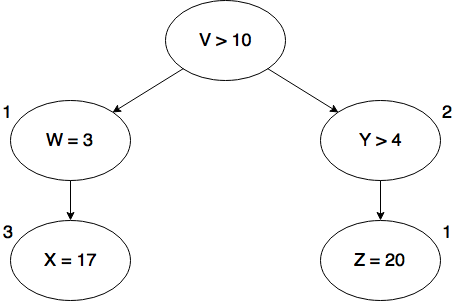
\includegraphics[width=3in]{SCCP.png} 
   \caption{Jerarqu\'ia de agentes}
   \label{fig:sccptree}
\end{figure}

Se puede utilizar un proceso de la forma $\sfunc{\tell(m)}_i$ para representar un mensaje $m$ para un agente $i$. De forma que, el proceso $\sfunc{\tell(T=51)}_1$ agregara esa restricci\'on al banco de informaci\'on del agente $1$. Un proceso de la forma $\sfunc{\ask Z>10 \rightarrow S>3}_2$ no puede evolucionar debido a que no es posible derivar $Z>10$ del banco de informaci\'on del agente $2$ (i.e., $Y<0$). Mientas que el proceso $\sfunc{\sfunc{\ask Z>10 \rightarrow S>3}_1}_2$ si puede evolucionar puesto que $Z>10 \sqsubseteq Z=20$. Un proceso de la forma $\sfunc{\sfunc{\ask Z>10 \rightarrow S>3}_1}_2 \| \sfunc{\tell(T=51)}_1$ ejecuta ambos procesos al mismo tiempo, de forma que el resultado es el descrito anteriormente. 

Si se define,
\\ $R \defsymbol \sfunc{ V = 42 }_3 \parallel T = 8 $, 
\\ $P \defsymbol \askp{ Y > 0 } { Z > 10 }$,
\\ $Q \defsymbol \askp{ T > 7 } { \sfunc{ S \neq 2 }_2 }$.

entonces, el proceso $S = \sfunc{R}_1 \parallel \sfunc{ P }_2 \parallel \sfunc{ Q }_1$ debe evolucionar tal como lo describe la Figura~\ref{fig:sccptree2}.

\begin{figure}[htbp] %  figure placement: here, top, bottom, or page
   \centering
   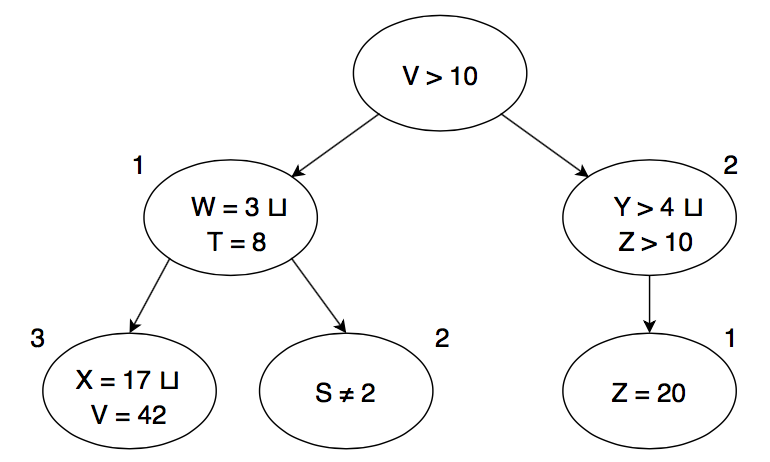
\includegraphics[width=3.5in]{SCCP-1.png} 
   \caption{Evoluci\'on del sistema}
   \label{fig:sccptree2}
\end{figure}

En el Cap\'itulo~\ref{chapter.rew} se muestra esta derivaci\'on utilizando la especificaci\'on formal.

